\documentclass[aps,prl,twocolumn,superscriptaddress]{revtex4-1}
\usepackage{graphicx}  % this is the up-to-date package for all figures
\usepackage{amssymb}   % for math
\usepackage{verbatim}  % for the comment environment
\usepackage{color}
\usepackage{subcaption} % for subcaptions on side-by-side figures
\usepackage{float}	% allows use of 'H' command
%\usepackage{hyperref}	% needed to add hyperlinks
%\hypersetup{
%  colorlinks=true,
%  linkcolor=blue,
%  filecolor=magenta,
%  urlcolor=cyan,
%}
\bibliographystyle{apsrev}


% these are some custom control of the page size and margins
% \topmargin= 0.2in  % these 1st two may be needed for some computers
% \textheight=8.75in
\textwidth=6.5in
%\oddsidemargin=0cm
%\evensidemargin=0cm

% this is where the actual document itself (rather than control statements) begins:

\begin{document}



\title{Evaluating the Pan-STARRS Variability Parameter}


\author{Daichi Hiramatsu}
\author{Corey Mutnik}
\email{dhiramat@hawaii.edu}
\email{cmutnik@hawaii.edu}
\affiliation{Department of Physics \& Astronomy, \\
University of Hawaii at Manoa,\\
2505 Correa Rd, Honolulu, HI, 96822, USA}
\altaffiliation{Observational Astronomy 301}



\begin{abstract}
\textbf{By Thursday (4/18) we need:} well thought out section titles and plots that show all the points we wanna make\\
~\\LS analysis on ATLAS Pathfinder Telescope data, verified PS variability criteria
\end{abstract}

\maketitle    




\section{Introduction}

\begin{itemize}
	\item{} why we care
	\item{} what made us care about this project
	\item{} NO structure / distance stuff (maybe put it in looking forward section at end)
	\item{} talk about PS catalog
	\item{} variability surveys (discuss other attempts to measure variables across the sky)
	\item{} why are variables interesting
	\item{} why do we want to find variables and care about where they are located
	\item{} Summary: we ran LS, analyzed stars, why did we do it all
	\item{} Mention what will be discussed: ``in section 2 we describe the observations we used...''
\end{itemize}

\section{ATLAS PathFinder 1 Observations}
\begin{itemize}
	\item{} we used data from ATLAS
	\item{} supplemented with ATLAS data [REF TONRY] (possibly make this s subsection)
	\item{} exposure time
	\item{} observation dates
	\item{} what was the weather like during observations
	\item{} PSF FWHM variations (only include if we discuss crowding)
	\item{} `we recieved the reduced image data from the ATLAS pipeline; which gave us RA, Dec, mag, etc...'
\end{itemize}

\subsection{Data}

\begin{itemize}
	\item{} how we got mags out of data...
	\item{} $l^{II}=202^{\circ}$
	\item{} $b^{II}=\pm5$
\end{itemize}

\begin{figure}[H]
	\centering
	%\caption{prob(f)}
	\textbf{Sorting Pattern}\par\medskip
		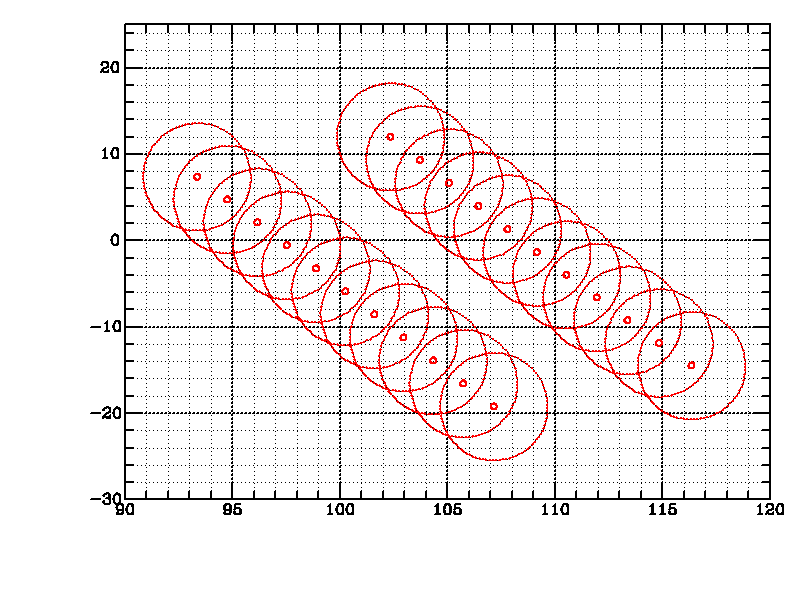
\includegraphics[width=3.35in]{figures/fromJT/sortedFOV.png}
	\caption{\it \small{Stars were grouped in the pattern shown (down the collected observations)}}
	\label{fig:sortpat}
\end{figure}

% from old paper
\iffalse
	\begin{itemize}
	 \item{} split observations into 1 $deg^2$ chunks
	 \item{} isolated groups s.t. each one is a star with 12 or more obs
	 \item{} $--$ more than 12 detections to be a star
	 \item{} $--$ any sq deg that has more than one star
	 \item{} this reduced 1300 $deg^2$ observation data down to ~300
	 \item{} before variability params: 1531417 stars in field
	 \item{} for variability parameters
	 \item{} $--$ log(average(upper quartile)) - log(average(lower quartile))
	 \item{} $--$ expect variation to go at .2* mag (from sqrt noise)...so subtract .2mag to get the logritmic statistic
	 \item{} sorted biggest (most variable?) to smallest (least variable?)
	 \item{} ran LS on 80,000 most variable stars, rather than full star groupings (over 1million)
	\end{itemize}
\fi



\section{Constructing Stellar Light Curves}
%\section{Constructing LightCurves for Stars}

% check out resource:
% https://www.aavso.org/lcg

\begin{itemize}
	\item{} how we selected stars (12+ obs, 1x1 deg$^2$, etc)
\end{itemize}



\section{Lomb-Scargle: Identifying Stellar Variability}
%\section{Identifying Variable Stars Using Lomb-Scargle}
\begin{itemize}
	\item{} extract variability from LS
	\item{} describe how it works and why we used LS
	\item{} major aliasing at 1 day and 0.5 day periods
	\item{} things that fall at at -50 (in Figure~\ref{fig:quartiles}) means that those are VERY probably variable stars
	\item{} roughly \_\_\_\_\_ stars fell at -50 in Figure~\ref{fig:quartiles}
	\item{} 320,000 stars tested for variability
	\item{} other stars (outside of 320,000) are statistically unlikely to be variable
\end{itemize}

\begin{figure}[H]
 \centering
 %\caption{prob(f)}
 \textbf{prob(f)}\par\medskip
 	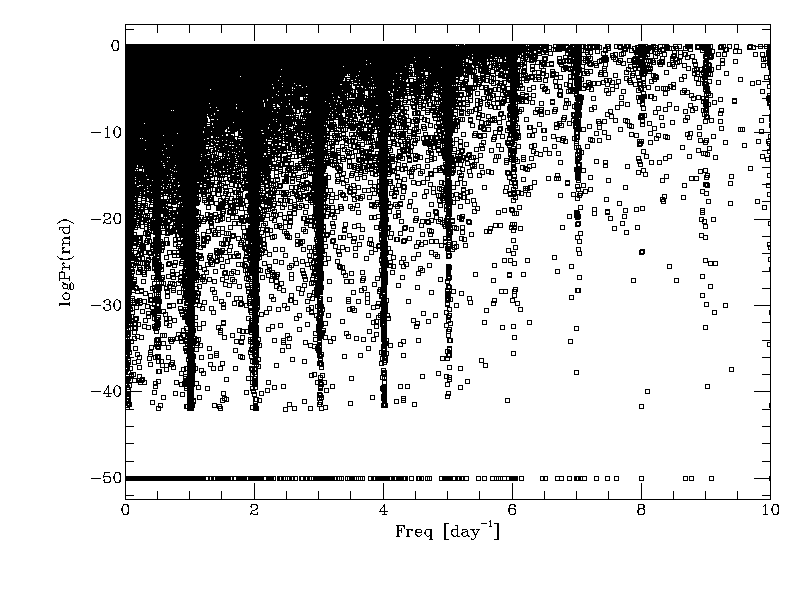
\includegraphics[width=3.35in]{figures/fromJT/probf.png}
 \caption{\it \small{prob(f) of 80,000, most variable, stars LS was run on}}
 \label{fig:quartiles}
\end{figure}




\section{Results}
\begin{itemize}
	\item{} compare with PS
	\item{} density/distribution of variables in sky
	\item{} (what LS gave us for our catalog)
	\item{} put a table with ~5 stars, to show off part of catalog
\end{itemize}

% From old paper
\iffalse
	\subsection{Simbad Completeness}
	\begin{itemize}
		\item{} Pull established RR list from Simbad
		\item{} Pull other variable data from simbad, too
		\item{} Compare list of observed RR to catalogs
		\item{} Is anyone actually reading this outline, this bullet point serves no purpose
		\item{} Wow, its sad how little Jeff did since class began (especially after JT gave him the code to do it a month ago) - 6 obs x 4 nights = January-April work period haha
		\item{} Establish completeness with Simbad
	\end{itemize}	
\fi


\begin{figure}[H]
	\centering
		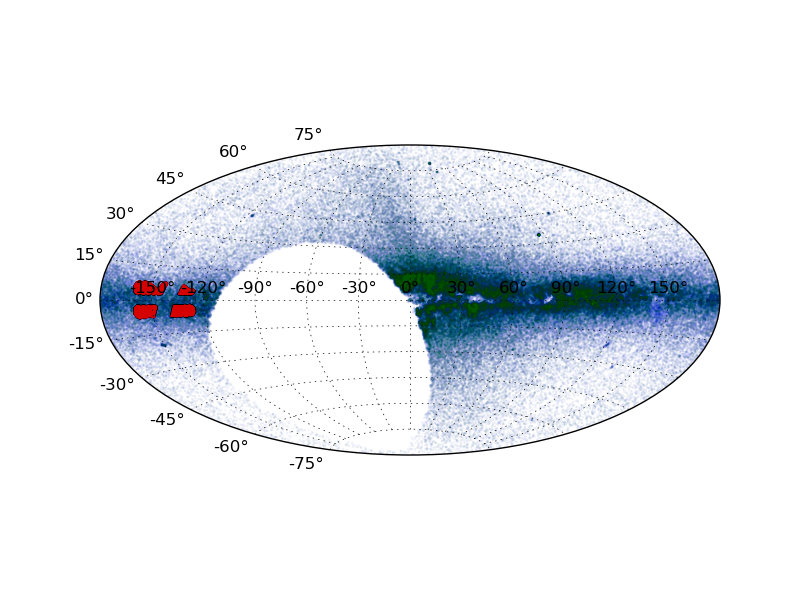
\includegraphics[width=3.35in]{figures/aitoff/Obs_PS_lsum_aitoff_map.png}
		\caption{\it \small{Aitoff projection of observed and PS RR Lyrae candidates.  Blue are candidates from PS that >= 0.05, green are PS candidates that >= 0.2., observed data in red.}}%
	\label{fig:aitoff_nosimbad}
\end{figure}


\section{Discussion}
\begin{itemize}
	\item{} Evaluation of PS criteria
	\item{} what went wrong
	\item{} what could have gone better
	\item{} future outlook
	\item{}~~~we could map spiral arms using x y and z
\end{itemize}

	

\begin{figure}[h!]
	\centering
	\begin{subfigure}{.5\textwidth}
	  \centering
	  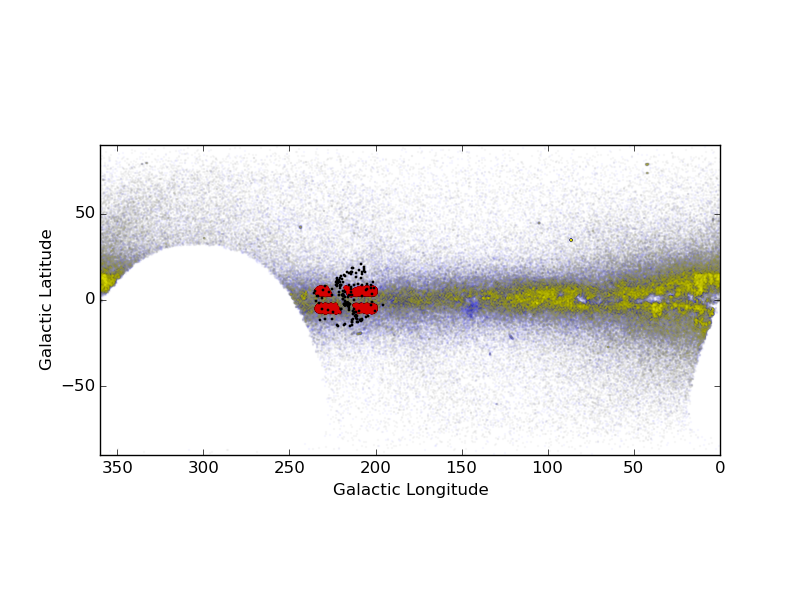
\includegraphics[width=1\linewidth]{figures/aitoff/simbad_alpha_is_1.png}
	  \caption{\it \small{Aitoff map.}}
	  \label{fig:aitoff_map_simbad}
	\end{subfigure}%
	\begin{subfigure}{.5\textwidth}
	  \centering
	  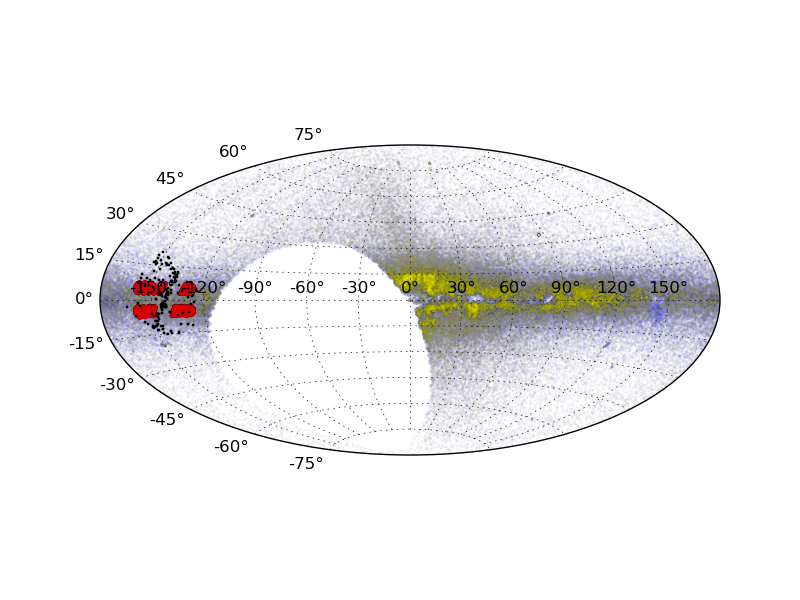
\includegraphics[width=1\linewidth]{figures/aitoff/Obs_PS_sim_lsum_aitoff_map.png}
	 \caption{\it \small{Aitoff projection}}%
	 \label{fig:aitoff_projection_simbad}
	\end{subfigure}
	\caption{\it \small{Aitoff projection of observed and PS RR Lyrae candidates.  Blue are candidates from PS that >= 0.05, yellow are PS candidates that >= 0.2., observed data in red, simbad in black.}}
	\label{fig:aitoff_simbad}
\end{figure}	


\section{Summary and Conclusions}
~[TALK ABOUT IT]



\setlength{\parindent}{0cm}

\begin{thebibliography}{99}  % the trailing 99 controls some obscure format--just use

%\bibitem{Sch_eq} Weisstein, Eric W. ``Schr\"{o}dinger Equation."

\end{thebibliography}


\end{document}

